\documentclass[10pt,times]{beamer}
\usepackage{amsfonts}
\usepackage{amsmath}
\usepackage{amssymb}
\usepackage{mathptmx}

\usepackage{color}
\usepackage{minted}
\usepackage{hyperref}
\usepackage{multicol}
\usepackage{tabularx}
\usepackage{booktabs}
\usepackage{menukeys}

% Stolen from John Miller's LaTeX course
\newcommand{\bftt}[1]{\textbf{\texttt{#1}}}
\newcommand{\comment}[1]{{\color[HTML]{008080}\textit{\textbf{\texttt{#1}}}}}
\newcommand{\cmmd}[1]{{\color[HTML]{008000}\bftt{#1}}}
\newcommand{\bs}{$\backslash$}
\newcommand{\cmdbs}[1]{\cmmd{\bs#1}}
\newcommand{\lb}{{\char'173}}% Left brackets -> {
\newcommand{\rb}{{\char'175}}% Right brackets -> }
\newcommand{\cmdbegin}[1]{\cmdbs{begin\lb}\bftt{#1}\cmmd{\rb}}
\newcommand{\cmdend}[1]{\cmdbs{end\lb}\bftt{#1}\cmmd{\rb}}



% this is where the example source files are loaded from
% do not include a trailing slash
\newcommand{\wllogo}{\textbf{Overleaf}}
\newcommand{\fileuri}{https://raw.githubusercontent.com/kks32/latex-course/master/exercises/}
\newcommand{\wlserver}{https://www.overleaf.com}
\newcommand{\wlnewdoc}[1]{\wlserver/docs?snip\_uri=\fileuri#1\&splash=none}

\def\tikzname{Ti\emph{k}Z}


% stolen from minted.dtx
\newenvironment{exampletwoup}
  {\VerbatimEnvironment
   \begin{VerbatimOut}{example.out}}
  {\end{VerbatimOut}
   \setlength{\parindent}{0pt}
   \fbox{\begin{tabular}{l| l}
   \begin{minipage}{0.55\linewidth}
     \inputminted[fontsize=\small,resetmargins]{latex}{example.out}
   \end{minipage} &
   \begin{minipage}{0.35\linewidth}
     \input{example.out}
   \end{minipage}
   \end{tabular}}}

\newenvironment{exampletwouptiny}
  {\VerbatimEnvironment
   \begin{VerbatimOut}{example.out}}
  {\end{VerbatimOut}
   \setlength{\parindent}{0pt}
   \fbox{\begin{tabular}{l|l}
   \begin{minipage}{0.55\linewidth}
     \inputminted[fontsize=\scriptsize,resetmargins]{latex}{example.out}
   \end{minipage} &
   \begin{minipage}{0.35\linewidth}
     \setlength{\parskip}{6pt plus 1pt minus 1pt}%
     \raggedright\scriptsize\input{example.out}
   \end{minipage}
   \end{tabular}}}

% ******************************** Meta-data ***********************************
\mode<presentation>
{
  \usetheme{Madrid}
  \setbeamercovered{transparent}
}


\usepackage{caption}
\captionsetup{font=scriptsize, labelfont=scriptsize, justification=centering}

\title{Writing papers and thesis using \LaTeX2e}

\author {Krishna Kumar \inst{*}\thanks{kks32@cam.ac.uk} }

\institute[ University of Cambridge ] % (optional, but mostly needed)
{
  \inst{1}%
  King's College\\
  University of Cambridge
}

\date[LaTeX course 2014] % (optional, should be abbreviation of conference name)
{\LaTeX for Beginners}


% Delete this, if you do not want the table of contents to pop up at
% the beginning of each subsection:
%\AtBeginSubsection[]
%{
%  \begin{frame}<beamer>{Outline}
%    \tableofcontents[currentsection,currentsubsection]
%  \end{frame}
%}


% If you wish to uncover everything in a step-wise fashion, uncomment
% the following command: 

% \beamerdefaultoverlayspecification{<+->}

\subtitle{Part II: Writing papers and thesis using \LaTeX}
%***************************** Title page **************************************
\begin{document}
\begin{frame}
  \titlepage
\end{frame}
%*******************************************************************************
%**************************** Introduction *************************************
%*******************************************************************************
\section{Graphics}

%*******************************************************************************
%******************************* Frame *****************************************
%*******************************************************************************
\begin{frame}[fragile]{Figures}
\begin{itemize}
\item \LaTeX can be easily extended using a \emph{package} to typeset images.

\item To use graphics in your \LaTeX document use \cmdbs{usepackage\{graphicx\}}

\item Always use relative scaling to specify the width of the figure, i.e., 

\cmmd{[width = 0.75\bs textwidth]}

\item Never ever use absolute values to scale your images!

\item Set either the width or the height of the image. Or use \cmmd{scale}

\end{itemize}
\begin{exampletwoup}
\begin{figure}

\includegraphics[width=0.75\textwidth]
                           {figs/minion}
\end{figure}
\end{exampletwoup}
\end{frame}


%*******************************************************************************
%******************************* Frame *****************************************
%*******************************************************************************
\begin{frame}[fragile]{Figures}
\begin{itemize}
\item For captioning a figure, you can use \cmdbs{usepackage\{caption\}}

\item tweak the location, label, separator: \cmmd{[labelsep=space, 
tableposition=top]\{caption\}}

\item I prefer to centre the figure. To do that use \cmdbs{centering}

\item You can use \cmmd{\~\bs cref\{fig:minion\}} to cross reference the figure.

\end{itemize}
\begin{exampletwoup}
\begin{figure}
\centering

\includegraphics[width=0.75\textwidth]
                           {figs/minion}
\caption[Minion]{
	Dave the Minion from Despicable Me!}
\label{fig:minion}
\end{figure}
\end{exampletwoup}
\end{frame}

%*******************************************************************************
%******************************* Frame *****************************************
%*******************************************************************************
\begin{frame}[fragile]{\bs begin[option]\{figure\}}
\renewcommand{\arraystretch}{1.5}
\begin{tabularx}{\textwidth}{l X}
\toprule
\textbf{Parameter} &	\textbf{Position} \\ \midrule
h &	Place the float here, i.e., approximately at the same point it occurs in 
the source text (however, not exactly at the spot) \\
t &	Position at the top of the page. \\
b &	Position at the bottom of the page. \\
p &	Put on a special page for floats only. \\
! &	Override internal parameters LaTeX uses for determining "good" float 
positions. \\
H &	Places the float at precisely the location in the LaTeX code. Requires the 
float package. This is somewhat equivalent to h! \\ \bottomrule
\end{tabularx}
\end{frame}

%*******************************************************************************
%******************************* Frame *****************************************
%*******************************************************************************
\begin{frame}[fragile]{Subcaption}

I can cite Wall-E (see~\cref{fig:WallE}) and Minions in despicable me 
(\cref{fig:Minnion}).~\Cref{fig:animations} lets me cite the whole figure.

\begin{exampletwouptiny}
\begin{figure}
  \centering
  \begin{subfigure}[b]{0.3\textwidth}
    
\includegraphics[width=\textwidth]
			    {figs/TomandJerry}
    \caption{Tom and Jerry}
    \label{fig:TomJerry}   
  \end{subfigure}             
  \begin{subfigure}[b]{0.3\textwidth}
    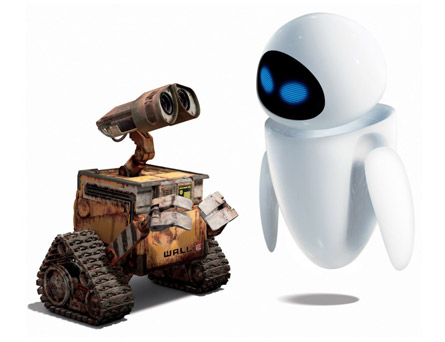
\includegraphics[width=\textwidth]{figs/WallE}
    \caption{Wall-E}
    \label{fig:WallE}
  \end{subfigure}             
  \begin{subfigure}[b]{0.3\textwidth}
    
\includegraphics[width=\textwidth]{figs/minion}
    \caption{Minions}
    \label{fig:Minnion}
  \end{subfigure}
  \caption{Best Animations}
  \label{fig:animations}
\end{figure}

\end{exampletwouptiny}


\end{frame}


\end{document}
